\documentclass[../../DD.tex]{subfiles}
\begin{document}
\section{C-IDM}
	The first Kind of topic that we encounter in the structure of the model is \textit{Musical Instrument}. This entity represents the instruments that are relevant for \textit{Lemon Peel} association. They are all instruments born in Italy, and each one has two charateristics that represent the region where it was born and the type of the instrument, known as its classification. A \textit{Musical Instrument} is related to the ones of the same type of from the same region.
	\newline
	The core of the model is represented by three main multiple topics, related to each other, that are \textit{Course}, \textit{Event} and \textit{Person}. A \textit{Course} represents the activity where the students can learn about regional folk songs or how to play a specific instrument. Due to their simplicity, some folk \textit{Musical Instruments} might not have a dedicated course, and there are no courses related to more than one instrument. Every course is held by at least a teacher (\textit{Person}) and might be presented in one or more Events.
	\newline
	The \textit{Events} are organized by \textit{Lemon Peel} association to let people know about its main goal or to present specific \textit{Courses} to attract more new musicians. There might be \textit{Events} to show what the students have accomplished during the season; in this case no \textit{Course} is related to them. An \textit{Event} is organized by exactly one \textit{Person}, that can be contacted to have specific information about it. 
	\newline
	\textit{Person} kind of topic include all the teachers who hold at least one \textit{Course}. A \textit{Person} can be expert of several musical fields; in this case she would be related to more than one \textit{Course}
	\newline
	Two single topics are included in the diagram: they are \textit{Association}, that is the \textit{Lemon Peel} entity, with its history, and \textit{Contacts}, that includes ways to contact the administrators of the association.
	\newline
	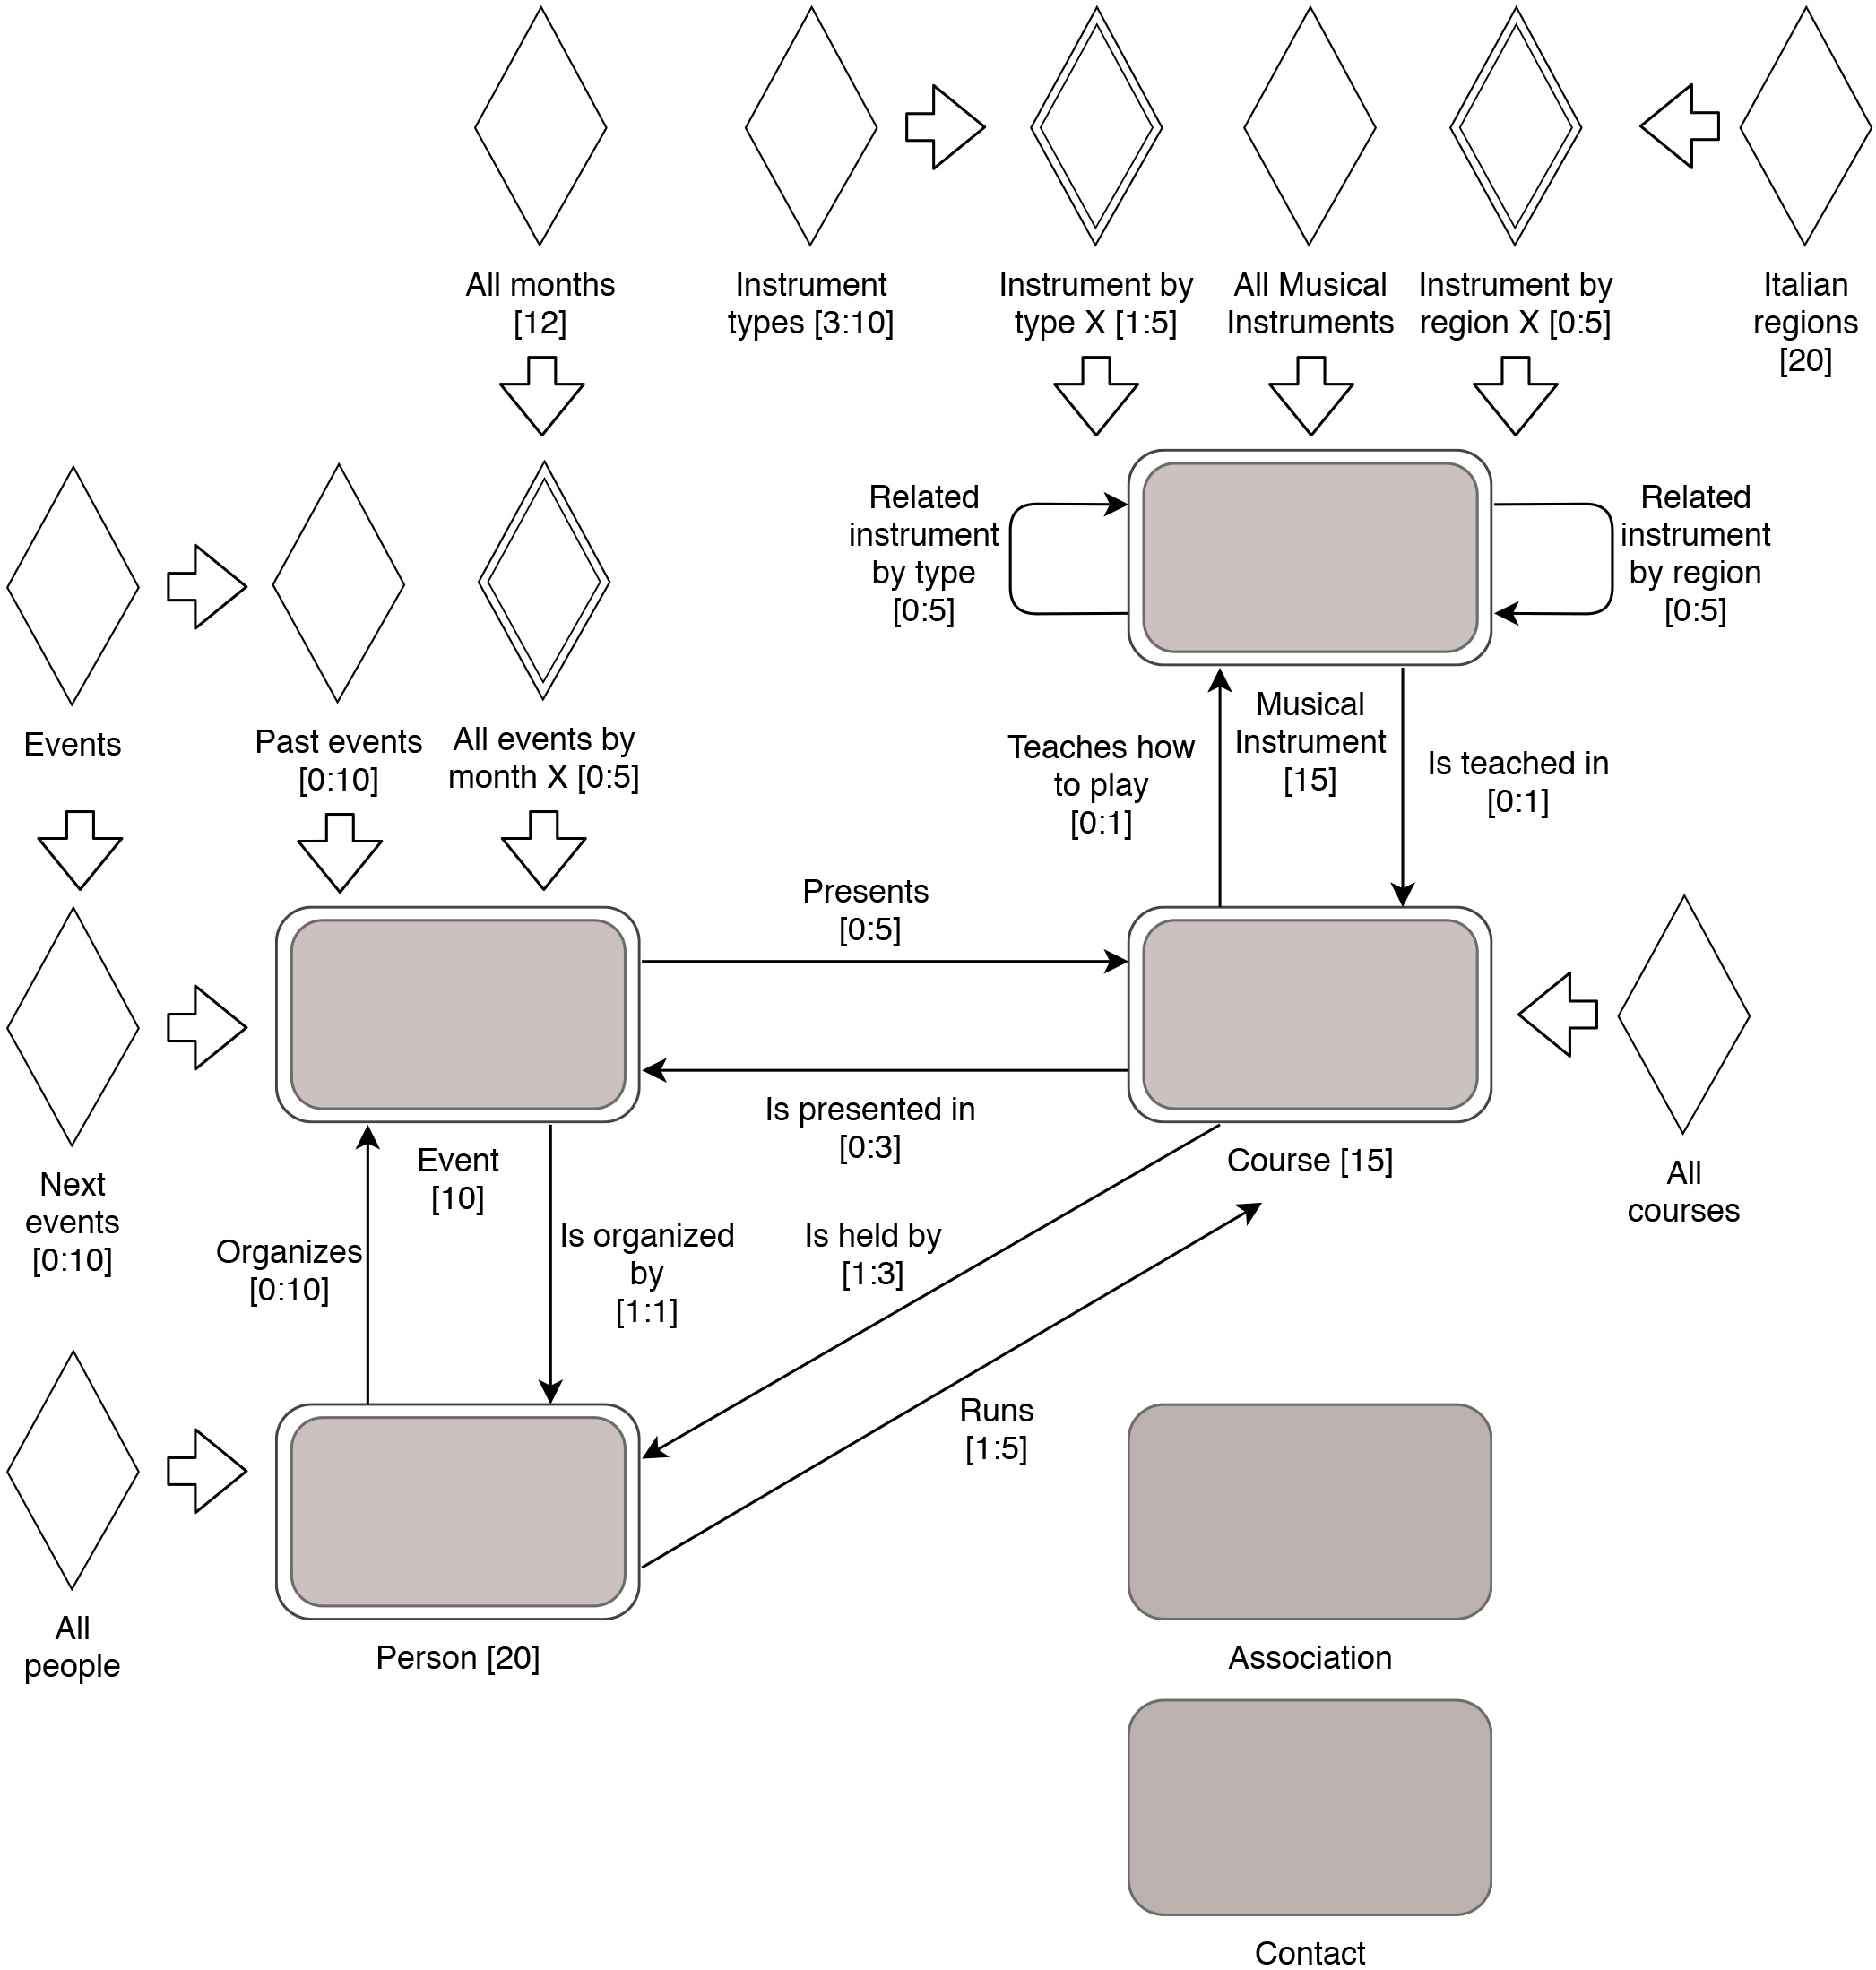
\includegraphics[width=\textwidth,height=\textheight,keepaspectratio]{IDM/C-IDM.jpg}
\end{document}
